\section{Preparation, Considerations and Initial Simulations}

\paragraph{}
To design a feasible commercial building incorporating low voltage DC electricity an approximate building size and layout was required. Through liaising with Geoff he suggested contacting QUT's Building Management Services department who have access to building schematics and load data. Geoff Woods and Norman Higgins provided electrical drawings, single line diagrams, architectural drawings and electrical specifications for analysis. Additionally, a computer login to the Electricity Management System (EMS) at QUT was created. This interface tracks all the electricity consumed from every meter on campus. The data is access through a interface closely linked with the single line diagrams of buildings including main switchboards (MSBs), distribution boards (DBs) and transformers. This information is critical to understanding optimal power system design. 

\paragraph{}
The EMS system additionally outlines how the PV system at QUT operates and what power it generates. The solar panels act as a load reducing generator rather than direct appliance powering. During the day the panels generate electricity and with a regulator and converter combination the DC generated power is converted to AC and fed into the University's power systems. The major difference between this design and the one which this project seeks to design is the panels will be directly powering loads. 

\subsection{Draft Floorplan}

\paragraph{}
Before the schematics and floor plans for QUT's buildings were made available, an approximate small office area was modelled in AutoCAD with offices of 5 \si{m^2}. The purpose of this simulation was to analyse approximate lighting loads for the environment.   

\begin{figure}[H]
\hfill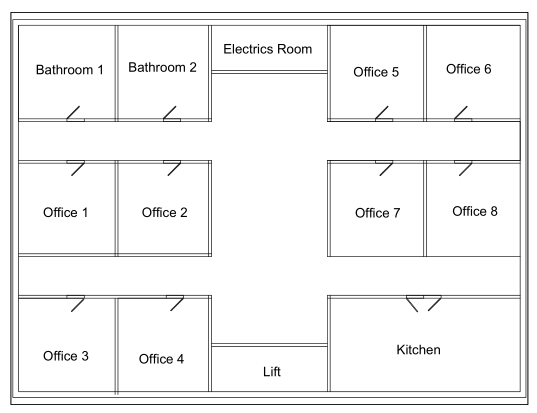
\includegraphics[width = 120mm]{images/Rough_Floorplan}\hspace*{\fill}
\caption{Temporary Office Floor Plan Design} 
\label{fig:RoughFloorplan}
\end{figure} 

\paragraph{}
After the initial room plans for created, the Australian Standards AS/NZS 1680.2.2 Interior and Workplace Lighting were consulted. 

\begin{table}[!ht]
\centering
\renewcommand{\arraystretch}{2}
\begin{tabular}{|l|c|}
\hline
\textbf{Area or Application} & \multicolumn{1}{l|}{\textbf{Lux Requirement}} \\ \hline
Rarely Visited & 40 \\ \hline
Storage Rooms or Change Rooms & 80 \\ \hline
Machine Work or Waiting Rooms & 160 \\ \hline
Food Preparation Room & 240 \\ \hline
Technical Office Room & 320 \\ \hline
Visually Difficult Work & 500 \\ \hline
\end{tabular}
\caption{Lighting Requires as per AS/NZS Standards \cite{StandardsAustralia2006}}
\label{LightingRequirements}
\end{table}